\subsection{Diseño de Multitoma Personalizada}

El kit requiere un sistema de distribución de energía eléctrica que alimente simultáneamente múltiples componentes con diferentes requerimientos de potencia. La ausencia de soluciones comerciales que satisfagan las necesidades específicas del proyecto motivó el diseño de una multitoma personalizada integrada a la plataforma base.

\subsubsection{Justificación del Diseño Personalizado}

La necesidad de una multitoma personalizada se fundamenta en las siguientes consideraciones operativas y técnicas:

\begin{itemize}
    \item \textbf{Limitación de tomas disponibles}: El laboratorio (Sala CAM) cuenta con número limitado de tomas de corriente por estación de trabajo, requiriendo centralización de alimentación
    
    \item \textbf{Fuentes existentes de dimensiones variables}: Los robots PhantomX Pincher poseen fuentes de alimentación de diferentes generaciones con geometrías no estándar
    
    \item \textbf{Reutilización de componentes}: Se busca aprovechar fuentes de alimentación existentes en el inventario del laboratorio
    
    \item \textbf{Nuevos requerimientos de alimentación}: La Raspberry Pi 5 requiere fuente USB-C Power Delivery no contemplada en kits originales
    
    \item \textbf{Flexibilidad operativa}: Se requiere conexión simultánea de robot, Raspberry Pi, bomba de vacío y equipo auxiliar (PC para desarrollo)
    
    \item \textbf{Control individual de energización}: Se necesitan interruptores independientes para cada subsistema como medida de seguridad y apagado de emergencia
\end{itemize}

Multitomas comerciales estándar no permiten:
\begin{itemize}
    \item Espaciamiento variable entre tomas para acomodar fuentes de geometrías irregulares
    \item Control individual mediante switches iluminados con identificación específica
    \item Integración mecánica con la plataforma base del kit
    \item Fusible de protección accesible para reemplazo
\end{itemize}

\subsubsection{Análisis de Requerimientos Eléctricos}

\paragraph{Consumo de Corriente por Subsistema}

El dimensionamiento eléctrico de la multitoma se basó en el consumo máximo de cada componente del kit:

\begin{itemize}
    \item \textbf{Raspberry Pi 5}: Fuente USB-C 5V/3A (consumo real máximo ~1.5 A @ 5V)
    \item \textbf{Robot PhantomX Pincher}: Fuente 12V/3A (consumo máximo con 5 servomotores bajo carga)
    \item \textbf{Bomba de vacío 370A}: Consumo directo 12V/1A máximo (0.42 A nominal)
    \item \textbf{Equipo auxiliar}: PC o monitor para desarrollo, estimado 3A máximo @ 120V
\end{itemize}

\paragraph{Corriente Total de Diseño}

Considerando operación simultánea de todos los subsistemas:

\begin{equation}
I_{total} = I_{RPi} + I_{robot} + I_{bomba} + I_{aux} = 1.5 + 3.0 + 1.0 + 3.0 = 8.5 \text{ A}
\end{equation}

Se establece corriente de diseño de 9.5 A con margen de seguridad del 12\%, valor confortablemente inferior al límite de 15 A de los componentes comerciales seleccionados.

\subsubsection{Cumplimiento Normativo de Cableado}

El cableado interno de la multitoma se diseñó siguiendo el Reglamento Técnico de Instalaciones Eléctricas (RETIE) vigente en Colombia \cite{RETIE2013}:

\begin{itemize}
    \item \textbf{Conductor de fase}: Cable rojo, calibre 14 AWG
    \item \textbf{Conductor neutro}: Cable blanco, calibre 14 AWG
    \item \textbf{Conductor de tierra}: Cable verde, calibre 14 AWG
\end{itemize}

El calibre 14 AWG (2.08 mm², capacidad 15 A) proporciona margen del 58\% respecto a corriente de diseño (9.5 A), garantizando operación sin calentamiento excesivo.

\subsubsection{Sistemas de Seguridad Eléctrica}

La multitoma incorpora múltiples niveles de protección:

\paragraph{Protección por Fusible}

\begin{itemize}
    \item Fusible tipo cartucho 15 A, 125 V AC
    \item Ubicado en conector de entrada AC-01
    \item Protección contra sobrecorriente por cortocircuito o falla de equipo
    \item Accesible para reemplazo sin desmontar carcasa
\end{itemize}

\paragraph{Control Individual por Subsistema}

Se implementaron tres switches balancín independientes:

\begin{enumerate}
    \item \textbf{Switch 1}: Robot PhantomX Pincher + Bomba de vacío (circuito común 12V)
    \item \textbf{Switch 2}: Raspberry Pi 5 (alimentación independiente 5V)
    \item \textbf{Switch 3}: Toma auxiliar para PC o equipo de desarrollo
\end{enumerate}

Cada switch cuenta con indicador luminoso (piloto LED integrado) que señaliza estado energizado/desenergizado.

\paragraph{Interruptor Maestro}

El conector de entrada AC-01 incorpora switch balancín maestro que energiza o desenergiza simultáneamente todos los circuitos derivados, funcionando como:
\begin{itemize}
    \item Apagado de emergencia de todo el sistema
    \item Desconexión completa durante almacenamiento o transporte
    \item Protección contra arranque inadvertido
\end{itemize}

\subsubsection{Dimensionamiento Geométrico}

El espaciamiento entre tomas se determinó mediante modelado 3D de las fuentes de alimentación existentes en el inventario del laboratorio. La Figura \ref{fig:fuentesVarias} presenta las cinco fuentes consideradas.

\begin{figure}[H]
    \centering
    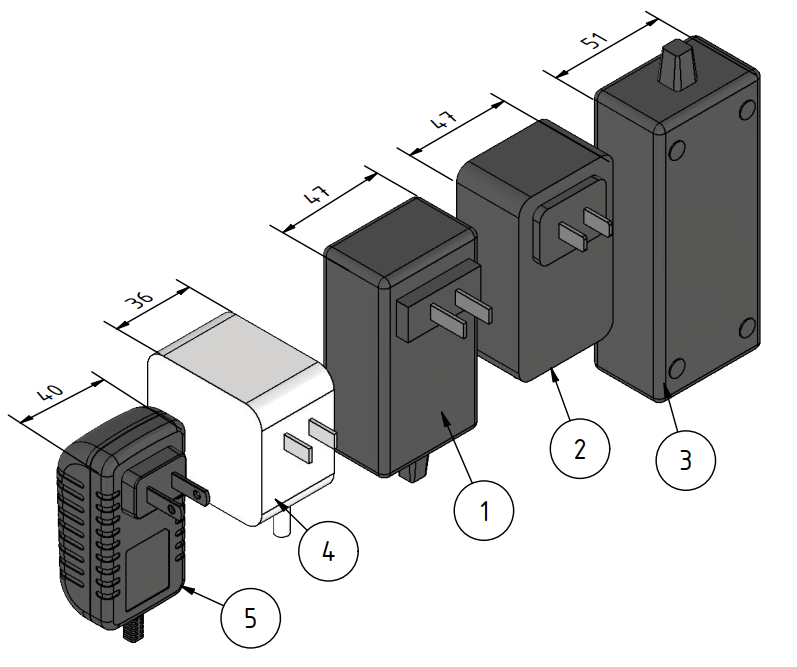
\includegraphics[width=0.7\textwidth]{06disenoConceptual/img/multitoma/fuentesVarias.png}
    \caption{Fuentes de alimentación modeladas para definir espaciamiento de tomas. (1) Fuente 12V/4A, largo 47 mm. (2) Fuente 12V/3A, largo 47 mm. (3) Fuente 12V/3A, largo 51 mm (geometría más grande). (4) Fuente 5V/5A USB-C para Raspberry Pi, largo 36 mm. (5) Fuente 12V/1A para bomba de vacío, largo 40 mm.}
    \label{fig:fuentesVarias}
\end{figure}

\begin{table}[H]
\centering
\caption{Fuentes de alimentación consideradas en el diseño}
\label{tab:fuentes_poder}
\small
\begin{tabular}{|c|l|c|}
\hline
\textbf{\#} & \textbf{Especificación} & \textbf{Largo (mm)} \\
\hline
1 & Fuente 12V/4A & 47 \\
2 & Fuente 12V/3A & 47 \\
3 & Fuente 12V/3A & 51 \\
4 & Fuente 5V/5A (USB-C) & 36 \\
5 & Fuente 12V/1A & 40 \\
\hline
\end{tabular}
\end{table}

\paragraph{Criterio de Espaciamiento}

Se estableció espaciamiento centro-a-centro de 26 mm para tres tomas principales, resultando en ocupación de 52 mm por toma (26 mm + 26 mm). Este espaciamiento acomoda la fuente más grande (51 mm) con holgura de 1 mm.

Para la toma destinada a la bomba de vacío (fuente de 40 mm), se redujo el espaciamiento a 22.5 mm centro-a-centro, optimizando el largo total de la multitoma.

\paragraph{Sistema de Identificación}

La carcasa incorpora marquillas grabadas en relieve que identifican la función de cada switch y toma:
\begin{itemize}
    \item "ROBOT" - Alimentación del manipulador PhantomX Pincher
    \item "VENTOSA" - Alimentación de bomba de vacío 370A
    \item "PI" - Alimentación de Raspberry Pi 5
    \item "PC" - Toma auxiliar de uso general
\end{itemize}

La Figura \ref{fig:vistasMultitoma} presenta vistas ortogonales de la multitoma con fuentes instaladas y sistema de identificación.

\begin{figure}[H]
    \centering
    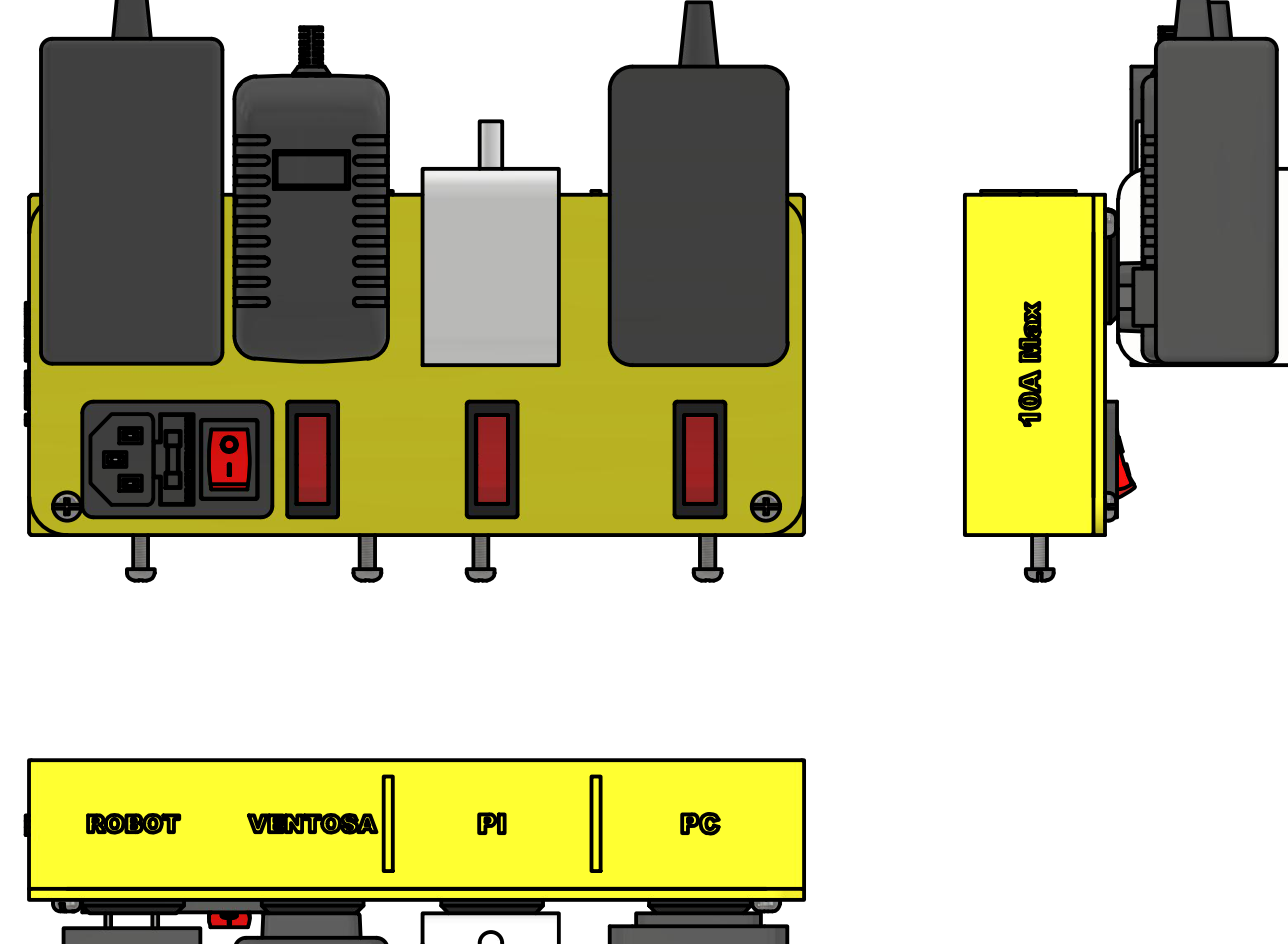
\includegraphics[width=0.95\textwidth]{06disenoConceptual/img/multitoma/vistasMultitoma.png}
    \caption{Vistas ortogonales de la multitoma con fuentes de poder instaladas. Vista frontal superior: Se observan cinco fuentes conectadas con espaciamiento optimizado. Los switches balancín (rojos) controlan energización individual. Vista lateral derecha: Perfil compacto con marquilla de capacidad máxima "10A Max". Vista inferior: Se muestran marquillas de identificación "ROBOT", "VENTOSA", "PI", "PC" que indican función de cada circuito. El conector AC-01 (izquierda) cuenta con switch maestro y fusible integrado.}
    \label{fig:vistasMultitoma}
\end{figure}

\subsubsection{Componentes del Conjunto}

El ensamble completo de la multitoma se presenta en la Figura \ref{fig:multitoma}.

\begin{figure}[H]
    \centering
    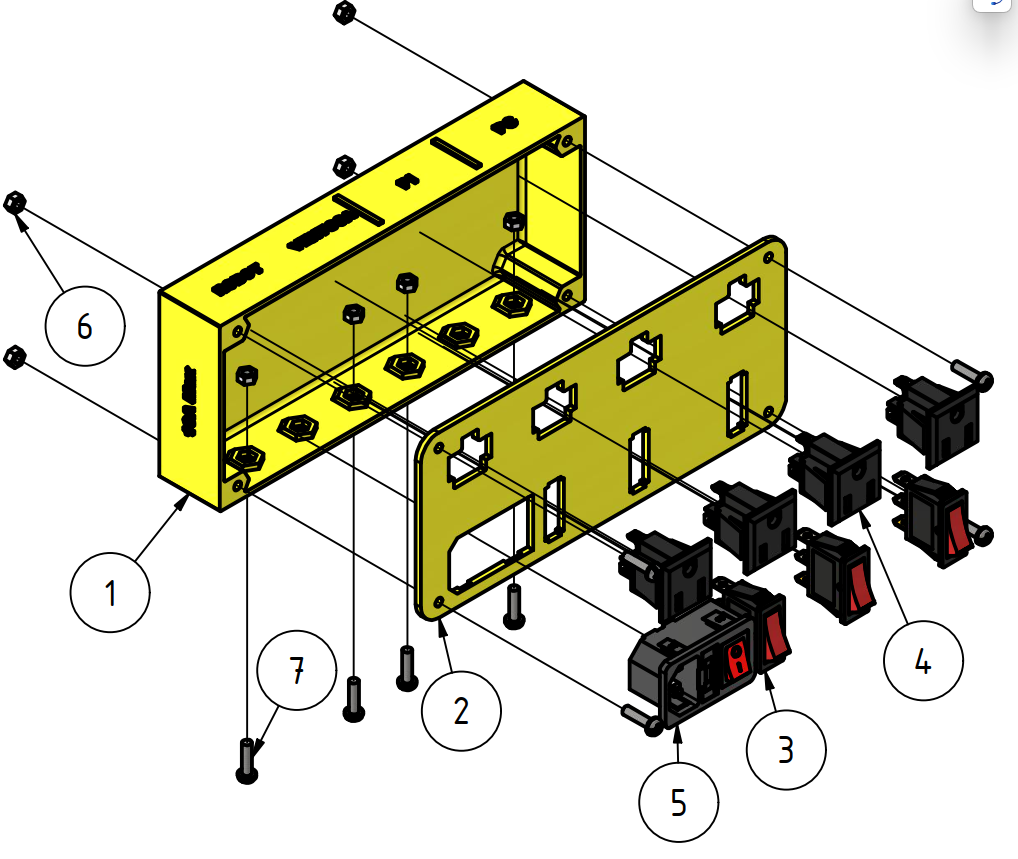
\includegraphics[width=0.85\textwidth]{06disenoConceptual/img/multitoma/multitoma.png}
    \caption{Ensamble explosionado de la multitoma personalizada. (1) Carcasa fabricada en PETG mediante FDM, incorpora cavidades para tuercas M4 cautivas en base. (2) Tapa de la multitoma con perforaciones para montaje de componentes eléctricos. (3) Switches balancín KCD3 de 3 pines con piloto LED integrado (3 unidades). (4) Tomas de corriente AC 125V/15A para montaje en panel (4 unidades). (5) Conector de entrada AC-01 para cable C13 con switch maestro y portafusible integrado. (6) Tuercas M4 cautivas para anclaje a plataforma (8 unidades). (7) Tornillos M4 × 15 mm para unión tapa-carcasa (8 unidades).}
    \label{fig:multitoma}
\end{figure}

\begin{table}[H]
\centering
\caption{Lista de materiales de la multitoma personalizada}
\label{tab:bom_multitoma}
\small
\begin{tabular}{|c|l|c|l|l|}
\hline
\textbf{\#} & \textbf{Componente} & \textbf{Cant.} & \textbf{Fabricación} & \textbf{Material} \\
\hline
1 & Carcasa de multitoma & 1 & FDM & PETG \\
2 & Tapa de multitoma & 1 & FDM & PETG \\
3 & Switch balancín KCD3 3 pines con piloto & 3 & Comercial & --- \\
4 & Toma AC 125V/15A montaje panel & 4 & Comercial & --- \\
5 & Conector entrada AC-01 cable C13 & 1 & Comercial & --- \\
6 & Tuerca M4 & 8 & Comercial & Acero \\
7 & Tornillo M4 × 15 mm & 8 & Comercial & Acero \\
8 & Fusible 15A 125V AC cartucho & 1 & Comercial & --- \\
9 & Cable cobre 14 AWG rojo × 1 m & 1 & Comercial & Cobre \\
10 & Cable cobre 14 AWG verde × 1 m & 1 & Comercial & Cobre \\
11 & Cable cobre 14 AWG blanco × 1 m & 1 & Comercial & Cobre \\
12 & Cable de poder C13 × 2 m & 1 & Comercial & --- \\
\hline
\end{tabular}
\end{table}

\textit{Nota: Los componentes 8-12 (cableado y fusible) no se representan en la Figura \ref{fig:multitoma} pues no eran necesarios para visualización del ensamblaje mecánico en modelo 3D.}

\subsubsection{Arquitectura de Ensamblaje}

El diseño de la multitoma emplea arquitectura de dos piezas principales:

\paragraph{Carcasa Base}

\begin{itemize}
    \item Fabricada en PETG por resistencia mecánica superior a PLA y menor deformación térmica
    \item Color amarillo para alta visibilidad de advertencias de seguridad
    \item Cavidades hexagonales en base inferior para alojar tuercas M4 cautivas
    \item Marquillas en relieve en superficie superior indicando posición de cada fuente
    \item Rebajes laterales para paso de cables de alimentación
\end{itemize}

\paragraph{Tapa con Componentes Eléctricos}

\begin{itemize}
    \item Todos los componentes eléctricos (switches, tomas, conector de entrada) se montan en la tapa
    \item Perforaciones dimensionadas para ajuste apretado de tomas AC (previene rotación)
    \item Cableado interno se realiza en tapa antes de cierre final
    \item Tapa se atornilla a carcasa mediante 8 tornillos M4 × 15 mm perimetrales
\end{itemize}

Esta arquitectura permite:
\begin{itemize}
    \item Ensamblaje y cableado de componentes eléctricos con carcasa abierta (acceso superior completo)
    \item Inspección visual de conexiones antes de cierre
    \item Mantenimiento o reemplazo de componentes sin desmontar multitoma de la plataforma
    \item Pruebas eléctricas previas al ensamblaje final
\end{itemize}

\paragraph{Anclaje a Plataforma Base}

Las tuercas M4 cautivas en la base de la carcasa permiten atornillar la multitoma a la plataforma MDF mediante tornillos que atraviesan desde la cara inferior de la plataforma. Esta configuración:
\begin{itemize}
    \item Integra mecánicamente la multitoma al kit
    \item Previene movimiento durante conexión/desconexión de fuentes
    \item Facilita gestión de cables entre multitoma y componentes
    \item Permite desmontaje completo para mantenimiento mayor
\end{itemize}

\subsection{Conclusión}

El diseño de la multitoma personalizada resuelve las limitaciones de soluciones comerciales mediante espaciamiento optimizado para fuentes de geometrías variables, control individual de energización de subsistemas con identificación clara, protección eléctrica mediante fusible accesible, y cumplimiento normativo RETIE en cableado interno. La arquitectura modular tapa-carcasa facilita ensamblaje, inspección y mantenimiento, mientras que la integración mecánica a la plataforma base proporciona estabilidad operativa y gestión ordenada de alimentación eléctrica del kit educativo.